\documentclass[12pt]{article}
\usepackage[a4paper,margin=0.8in]{geometry} % 明確設定四邊
\usepackage{fontspec}
\usepackage{xeCJK}
\usepackage{titling} % 預設標題下移0.6in
\usepackage{amsmath} % 數學方程式
\usepackage{graphicx} %圖片
\usepackage{float} % 在導言區 ,讓圖片強制插在原地
\usepackage{xcolor} %字體加入顏色
\usepackage{hyperref} % 引入網址
\usepackage{physics} % 物理符號
\usepackage{wrapfig} % 文字環繞圖片
\setmainfont{Times New Roman}
\setCJKmainfont{Kaiti TC}

\setlength{\droptitle}{-1in} % 上移標題0.6in
\title{TVD(總變差衰減)格式}
\author{3.assignment\_2.3.tex}
\begin{document} 
\maketitle 
\noindent (一)、方程式的空間二階精度TVD離散格式:(一般TVD(總變差衰減)格式)\\

對於不可壓縮理想氣體的二維穩態擴散對流方程,若取如下三項近似,則離散化後的二維擴散對流方程即為二維擴散對流方程的空間二階精度TVD離散格式:\\

\noindent (1)($M$($T$($f$($P$有限體積)的(邊界中心點))的(溫度))的(空間二階精度TVD格式)):
\begin{equation}
    \begin{split}
        T_{f} \approx T_{C} + \psi(r_{f})
        \cdot \frac{T_{D}-T_{C}}{2}
    \end{split}
\end{equation}

\noindent 其中,該格式的通量限制函數$\psi(r_{f})$需要坐落於TVD單調區域中,
$r_{f}$為通量限制函數的參數,$$r_{f} = \frac{T_{C}-T_{U}}{T_{D}-T_{C}}$$

\begin{figure}[H]
  \centering
  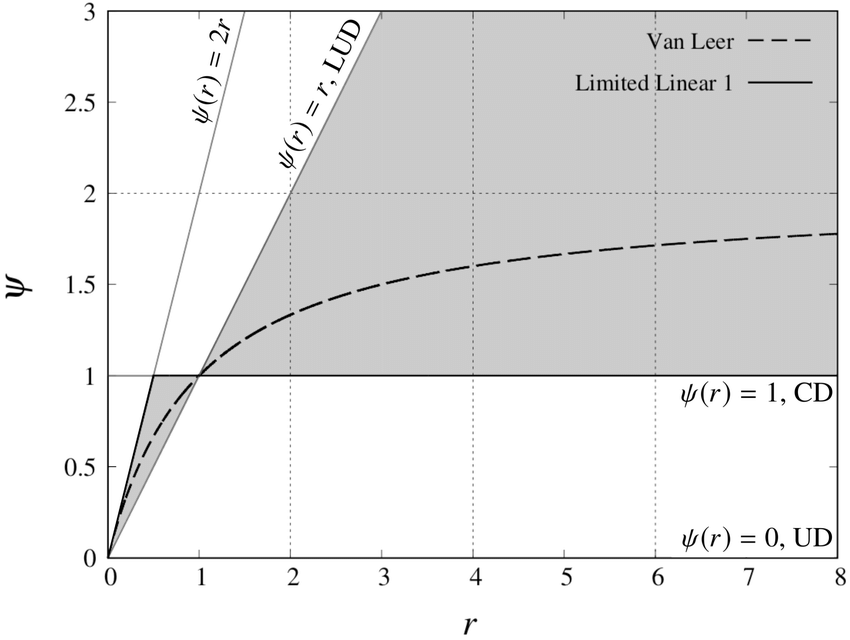
\includegraphics[scale = 0.3]{6.png}
  \caption{TVD單調區間,若坐落於此區域,則邊界上的對流通量的近似取值保持單調}
  \label{fig:TVD scheme }
\end{figure}


\noindent (二)、空間二階精度MINMOD離散格式:\\

空間二階精度MINMOD離散格式為一TVD格式,(1)空間二階精度MINMOD離散格式的通量限制函數$\psi(r_{f})$坐落於TVD(Total Variation Diminishing)(相鄰格點數值差總和遞減)單調區域中,且(2)
根據Van Leer等人的論證,空間二階精度MINMOD格式的通量限制函數必為空間二階精度SOU格式的
通量限制函數與空間二階精度中心差分格式的通量限制函數的線性組合。\\
\noindent 空間二階精度MINMOD離散格式的通量限制函數為:\\
\begin{equation}
    \begin{split}
        \psi(r_{f}) = max[0,min(1,r_{f})]\\
    \end{split}
\end{equation}
\noindent 其中,$r_{f}$為通量限制函數的參數,$$r_{f} = \frac{T_{C}-T_{U}}{T_{D}-T_{C}}$$且($C$計算點)為($C$($f$($P$有限體積)的(邊界點))的(上游計算點)),($D$計算點)為($D$($f$($P$有限體積)的(邊界點))的(下游計算點)),($U$計算點)為($U$($f$($P$有限體積)的(邊界點))的(上上游計算點))。\\

\noindent (1)當$r_{f} > 1$時,($L$($A$($E$($f$($P$有限體積)的(邊界點))的(傳輸變數))的(空間二階精度MINMOD格式))的(通量限制函數))-$\psi(r_{f}) = 1$,與($c$($C$($E$($f$($P$有限體積)的(邊界點))的(傳輸變數))的(空間二階精度CD格式))的(通量限制函數))重合。\\
\noindent (2)當$1>r_{f}>0$時,($L'$($A$($E$($f$($P$有限體積)的(邊界點))的(傳輸變數))的(空間二階精度MINMOD格式))的(通量限制函數))-$\psi(r_{f}) = r_{f}$,與($s$($S$($E$($f$($P$有限體積)的(邊界點))的(傳輸變數))的(空間二階精度SOU格式))的(通量限制函數))重合。\\
\noindent (3)當$r_{f} < 0$時,($L''$($A$($E$($f$($P$有限體積)的(邊界點))的(傳輸變數))的(空間二階精度MINMOD格式))的(通量限制函數))-$\psi(r_{f}) = 0$,與($u$($U$($E$($f$($P$有限體積)的(邊界點))的(傳輸變數))的(空間一階精度迎風格式))的(通量限制函數))重合。\\
\begin{equation}
\begin{split}
  &(1) \psi(r_{f}) = 1 ,\quad r_{f} > 1 \\
  &(2) \psi(r_{f}) = r_{f} ,\quad 1 > r_{f} > 0 \\
  &(3) \psi(r_{f}) = 0 ,\quad  r_{f} < 0
\end{split}
\end{equation}

\vspace{0.7em}
{\centering
\noindent 由此可知,空間二階精度MINMOD離散格式亦有6個邊界,9個角點需要討論,只是在不同範圍的$r_{f}$取值下,需要條件篩選。\\
}
\vspace{0.6em}
\noindent (二、1)、對流項中邊界中心點的溫度近似取值:\\
\noindent ($M$($T$($f$($P$有限體積)的(邊界中心點))的(傳輸變數))的(空間二階精度MINMOD格式)):\\
\begin{equation}
    \begin{split}
        T_{f} \approx T_{C} + \psi(r_{f})
        \cdot \frac{T_{D}-T_{C}}{2}
    \end{split}
\end{equation}
\noindent 其中,該格式的通量限制函數$$\psi(r_{f}) = max[0,min(1,r_{f})]$$
{\centering
上式坐落於TVD單調區域中\\}
\vspace{0.6em}
\noindent 因此,邊界中心傳輸變數近似格式有:
\begin{equation}
\begin{split}
  &(1) T_{f} = \frac{T_{C} + T_{D}}{2} ,\quad r_{f} > 1  ,\quad CD\mbox{格式}\\
  &(2) T_{f} = \frac{3}{2}T_{C} - \frac{1}{2}T_{U} ,\quad  1 > r_{f} > 0 ,\quad SOU\mbox{格式}\\
  &(3) T_{f} = T_{C} ,\quad  r_{f} < 0 ,\quad Upwind\mbox{格式}
\end{split}
\end{equation}

\noindent (二-2)、MINMOD離散格式中對方程式的三項近似:\\

\noindent (1)($M$($T$($f$($P$有限體積)的(邊界中心點))的(溫度))的(空間二階精度MINMOD格式))如(5)所示。\\
\noindent (2)($dT$($f$($P$有限體積)的(邊界中心點))的(溫度梯度))的近似取值採用二階精度中心差分。\\
\noindent (3)($G$($f$($P$有限體積)的(邊界中心點))的(擴散係數))的近似取值為該邊界點上游計算點的擴散係數$\alpha_{C}$與下游計算點的擴散係數$\alpha_{D}$之平均。\\
\vspace{0.7em}

\end{document}


